\section{More advanced exercises}
\subsection{GPS Data analysis}
\begin{figure}
\begin{center}
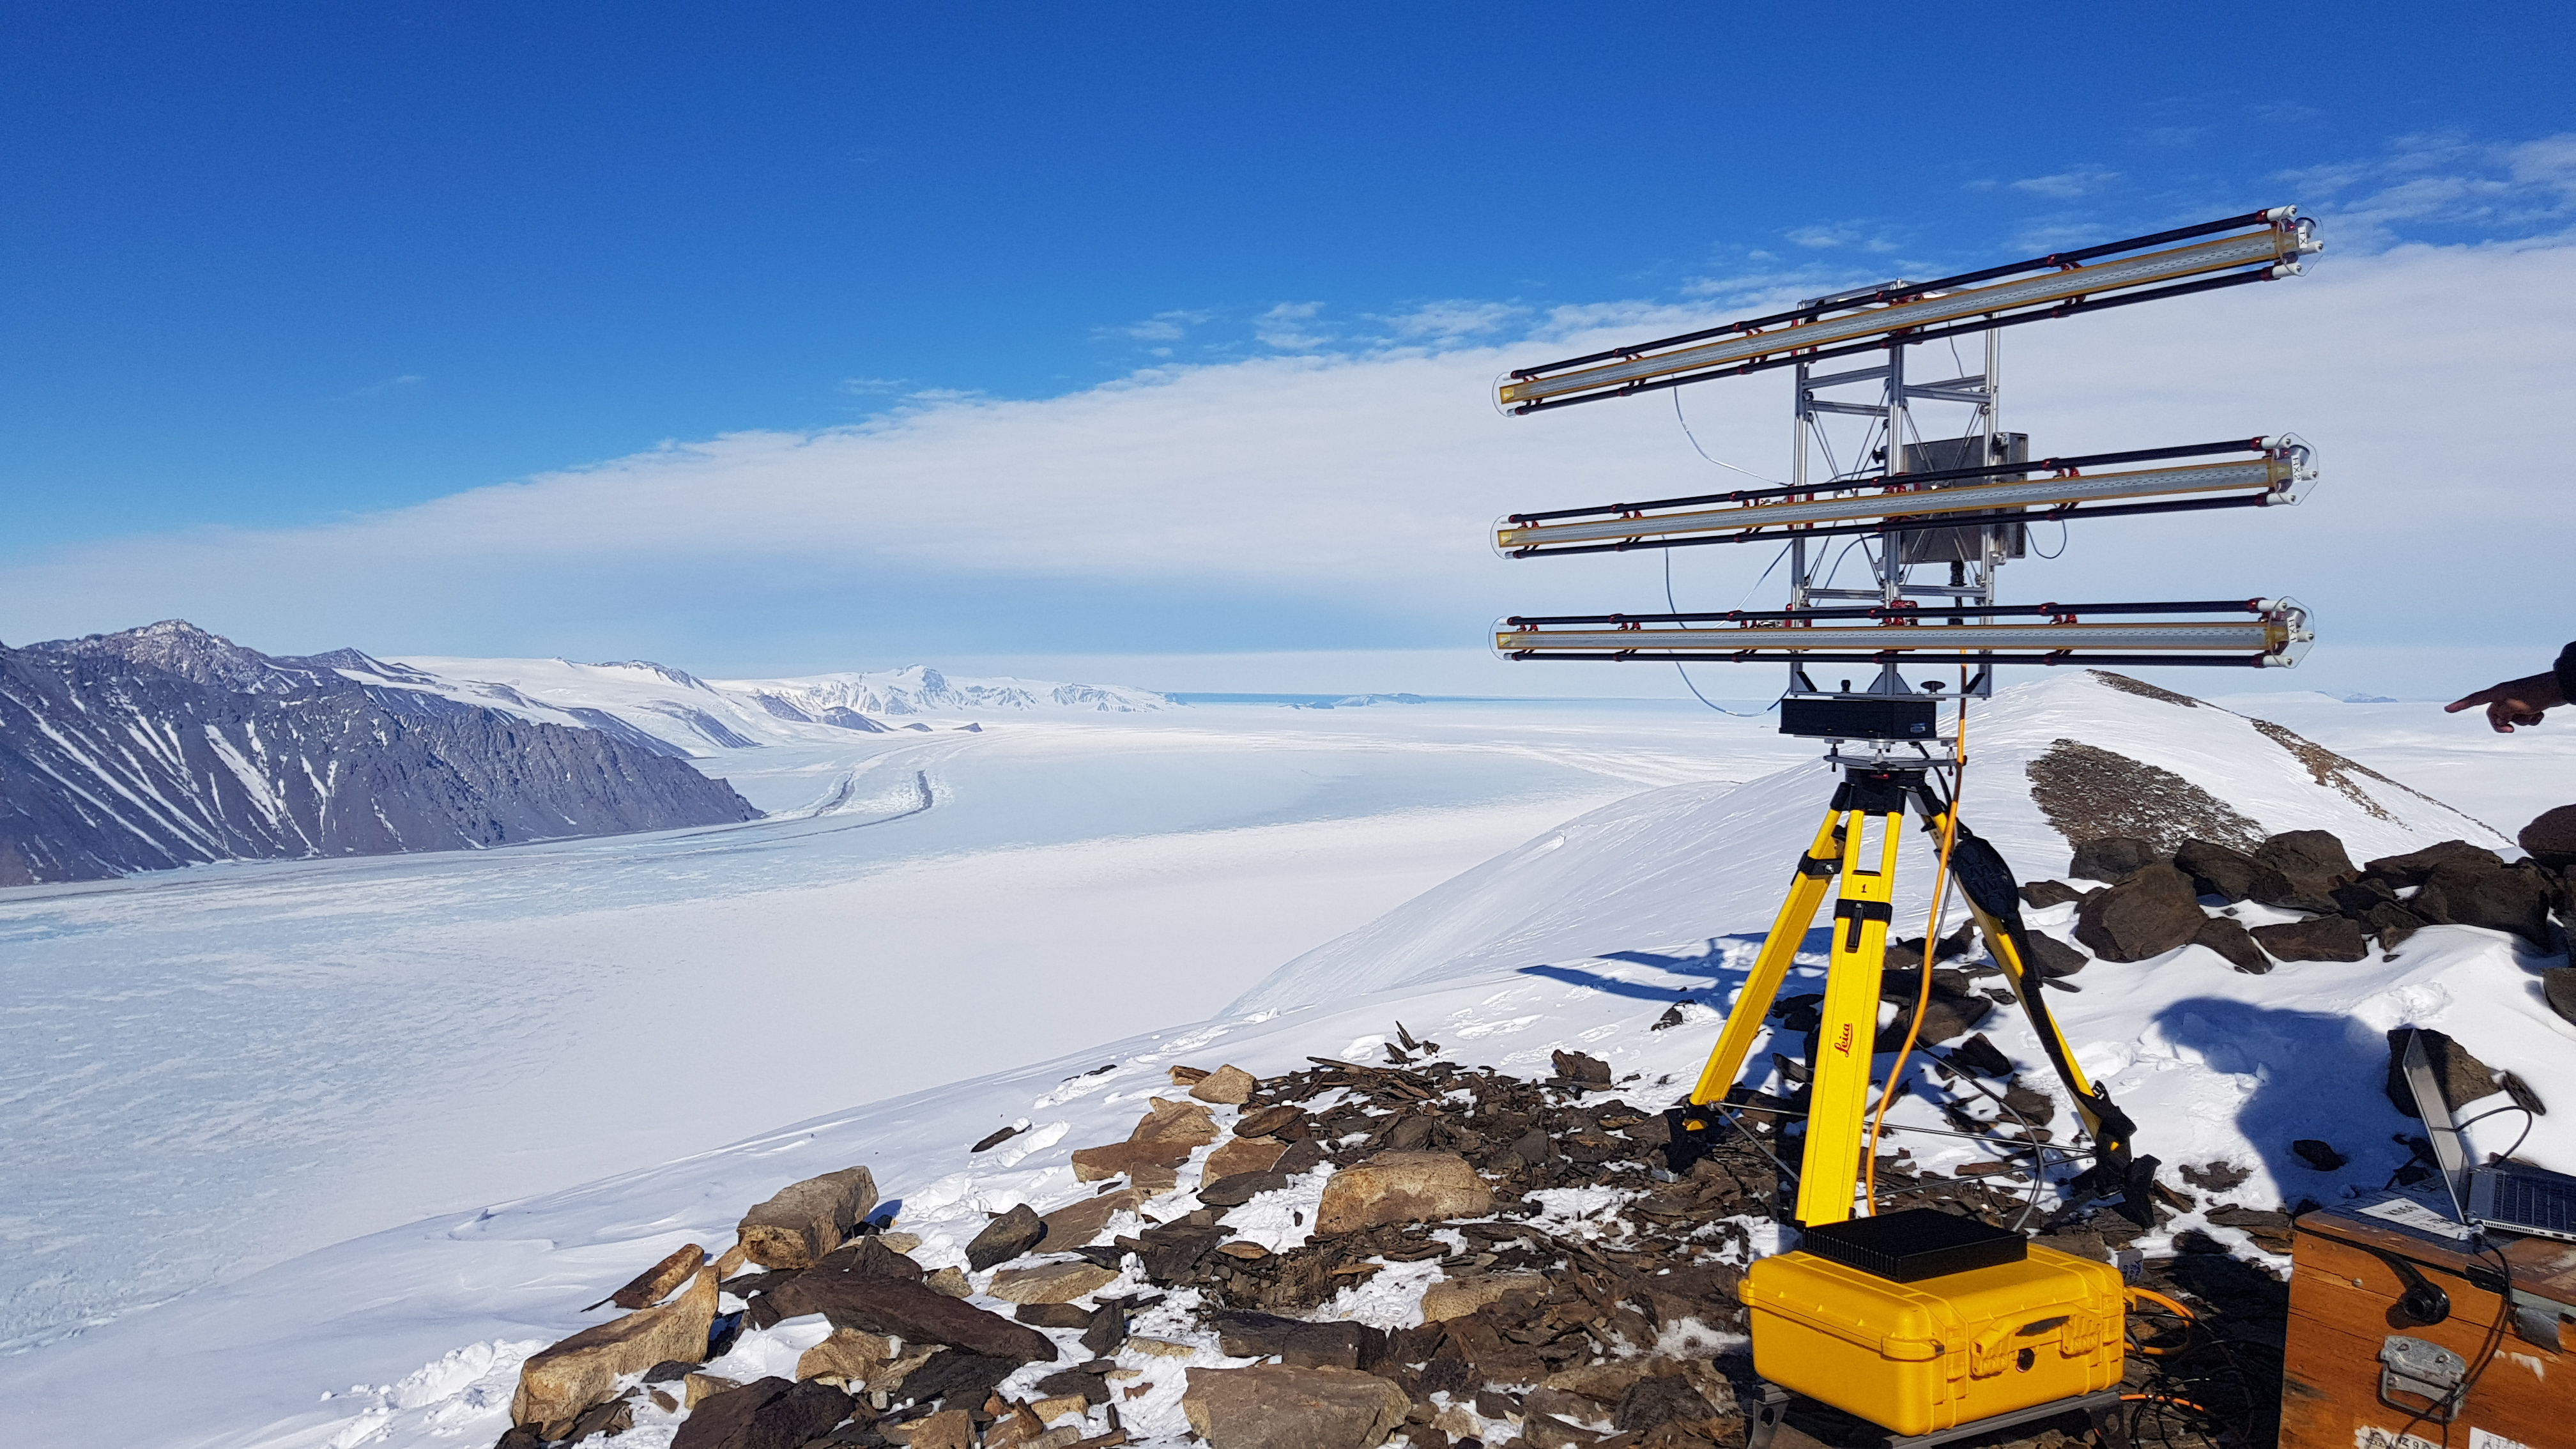
\includegraphics[width=15cm]{Figures/20181031_140359.jpg}
\caption{View downstream of Priestley Glacier. At the far end you can see the ocean. The ice starts to float on ocean water approximately at the end of the mountain chain located at the glaciers true left side.}
\end{center}
\end{figure}
Today's topic is focused on Antarctica. The data file \textit{XYShirase\_GPS\_Small.txt} is the output of GPS measurements located at Priestley Glacier feeding into the Nansen Ice Shelf. Ice shelves are the floating extensions of the Antarctic Ice Sheet. Beneath them is only water and consequently the ice lifts up and down with ocean tides. The data file contains 6 columns (1: Position in polar stereographic x, 2: Position in polar stereographic y, 3: Longitude, 4: Latitude, 5: Elevation, 6: Time). The polar stereographic projection (EPSG:3031) is a rectangular coordinate system with units meters (sort of comparable to UTM coordinates). The time is given in modified Julian days which are days since November 17, 1858 (just for information, not needed in exercise). Please complete the following tasks. Some are easier, some are harder.

\begin{itemize}
\item Visualize the movement of the GPS station in a x-y scatter plot (easy)
\item Visualize the vertical GPS position as a time series (easy). Which tidal  regime is visible here?
\item Calculate the mean horizontal GPS velocity in the observational period  Pythagoras is your friend. Always. (medium).
\item The vertical position has a fair amount of scatter. This is normal, as GPS measurements are about three times worse in the vertical compared to the horizontal direction. Smooth the data with your own moving average filter with variable window size. This filter should average the vertical position at time t as a mean value for a given number of positions recorded close to t. Assume that the data are regularly spaced in time. Cut-off the smoothed vector at the beginning and the end. It can be smaller than the data file (medium, involves for loops).
\item Find functions in python that  do a similar job and compare your results. (easy)
\item Discuss the pitfalls of filtering and suggest improvements. Memorize that a moving average filter is usually not the best way to go for noise reduction. Better options are weighted moving average or bandpass filters.
\item Design your own FIR low-pass filter, e.g., following \url{https://tomroelandts.com/articles/how-to-create-a-simple-low-pass-filter}. This is advanced and outside the scope of this course. Only do this if everything else is easy for you. We will not discuss the theory here.
\end{itemize}

\subsection{Cellular Automata: Abelian Sandpile Model}
Self-organized criticality is a fascinating subject that occurs in a number of geo- and environmental processes. Your job is to simulate an Abelian Sandpile Model which has in fact some quite realistic insights into the nature of landslides. The rules of this system are (Wikipedia entry has a more formal version of it):
\begin{itemize}
  \item Choose a random location on your grid and drop a grain of sand (i.e. add +1)
  \item Continue unless one of your grid points as more than 3 grains. 
  \item If a grid point as more than 3 grains then empty that cell, and distribute all grains to gridpoints in the surrounding (this is a landslide). Then continue.
  \item Grains fall of the boundaries are lost. 
\end{itemize}
Implement this set of rules on a grid and visualize its evolution.


\subsection{Cellular Automata: Langton's Ant as a 2D example}
Imagine you are in a 2D universe that is intially completely white on consists out of 100 x 100 cells that you can walk on. Your life depends on two rules only:

\begin{itemize}
    \item At a white square, turn 90 right, flip the color of the square, move forward one unit
    \item At a black square, turn 90 left, flip the color of the square, move forward one unit
\end{itemize}

Will you ever leave your world? The rules are simple enough, but an answer to this question is very difficult if not impossible. However, you can find the answer in Python. Go for it (with our help)! Cellular automata such as this have many applications in Geosciences. Another important model is, e.g., the sandpile model.
